% !TEX root = ../main.tex

This section will describe the implementation of the backend as well as the frontend. Implementation diagrams, code examples, and technical descriptions will be used. 

\subsection{Java Spring REST Backend}
To support the system functionality a Java RESTful service was developed using Spring. The reasoning behind using a REST backend is that the service can be consumed by any client that supports HTTP. Thus allowing for a web client as well as an android application to communicate with the backend. The endpoints for the service was implemented in accordance to the implementation class diagram \ref{fig:backend_class_diagram}. 

\begin{figure}[hbt]
\centering
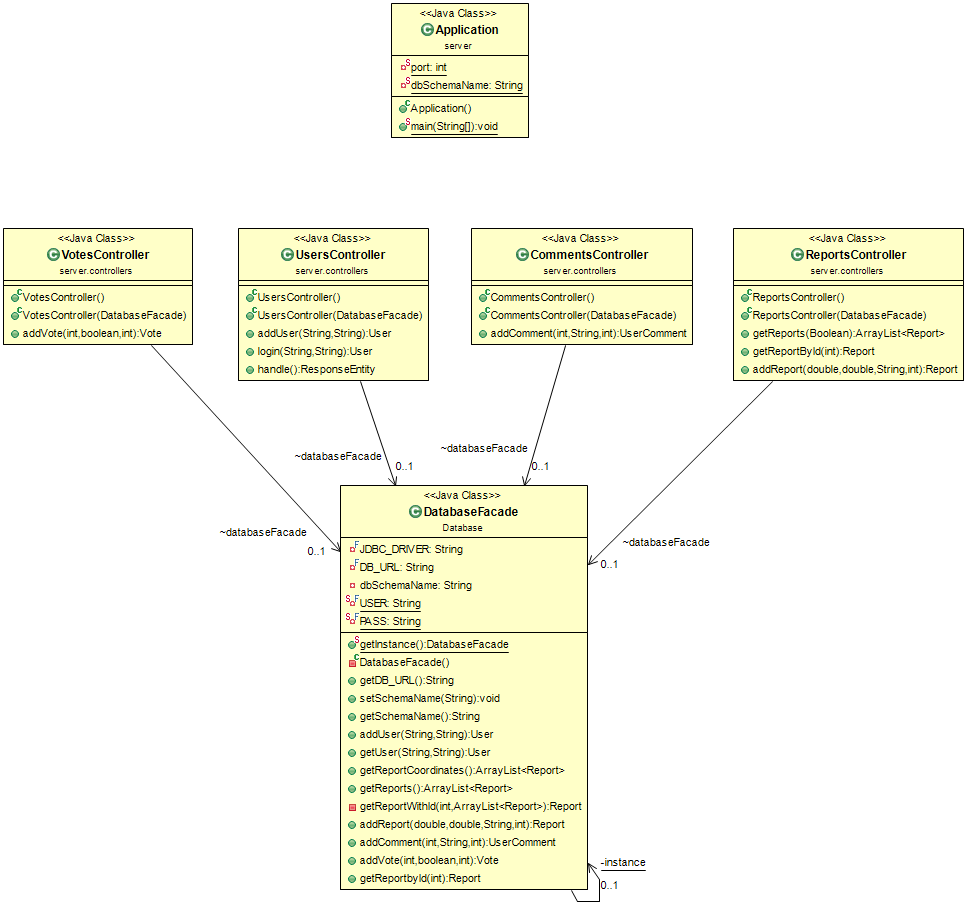
\includegraphics[width=\linewidth]{images/Class_backend_diagram}
\caption{Server side class diagram.}\label{fig:backend_class_diagram}
\end{figure}

\todo[inline]{explain the diagram in \autoref{fig:backend_class_diagram}}
\autoref{fig:backend_class_diagram} shows the classes implemented in the backend. All the controller have two constructors; an empty constructor and a constructor that takes a DatabaseFacade class as a parameter. This is used to enable unit testing of the REST controllers by allowing dependency injection to mock the database facade. The database facade contains the logic for communicating with a MySQL database using JDBC thus achieving persistence for the application. 

\begin{description}
\item [The VotesController] lets users add an up- or downvote to reports.
\item [The UsersController] lets unregistered users sign up and lets registered users login.
\item [The CommentsController] lets users add comments to reports.
\item [The ReportsController] lets users get all reports, get a report by id, and add a new report.
\end{description}

\begin{listing}[H]
\caption{Hello there}\label{lst:restController}
\todo[inline]{change the caption of Code Snippet \ref{lst:restController}}
\begin{minted}{java}
@RestController
@RequestMapping(value = "/api")
public class ReportsController {

    @RequestMapping(value = "/reports", params = {"only-coordinates"})
    public ArrayList<Report> getReports(@RequestParam(value="only-coordinates")
    Boolean onlyCoordinates) {
        if (onlyCoordinates) {
            return databaseFacade.getReportCoordinates();
        } else {
            return databaseFacade.getReports();
        }
    }
}
\end{minted}
\end{listing}

In Spring a REST endpoint is defined by using annotations. Specifically the annotation "\textit{@RestController}" is used to define an endpoint known as a  controller. This controller does not default to any URI, but another annotation is used for specifying the endpoint URI. The "\textit{@RequestMapping}" annotation is used for specifying URI's - the specific methods as well as the controller itself can use this annotation. All of the controllers maintain a reference to a database facade which is responsible for making the transactions with MySQL database to maintain persistent data.

\subsection{Databse}
The REST service is responsible for enabling HTTP access to the backend while the database facade is responsible for communicating with the MySQL database through JDBC. The database schema required to support the application is shown in figure \ref{fig:database_diagram}.

\begin{figure}[hbt]
\centering
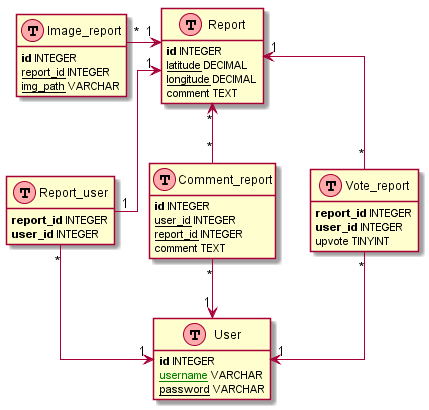
\includegraphics[width=.6\textwidth]{images/relational_model}
\caption{Relational Model that shows the database structure}\label{fig:database_diagram}
\end{figure}

The database diagram in figure \ref{fig:database_diagram} shows how the issue reports are connected to users and how the details of a report is interconnected. 

The \textbf{Image\_report} table contains a primary key \textit{id}, highlighted by underlining the column name, a foreign key \textit{id\_report}, highlighted by \textit{italic text}, and an \textit{img\_path} column. The \textit{img\_path} column is a string containing the relative path to an image file stored on the system. 

The \textbf{Comment\_report} table contains comments on reports submitted after the publishing of a report. The table contains two foreign keys that references the \textit{Report} and \textit{User} tables as well as a comment column.

The \textbf{Vote\_report} table contains the votes that users have cast on reports. The vote is saved as a TINYINT which is converted to a boolean value in Java. The table also contains two foreign keys - which is both primary keys as it is a weak entity - that references the \textit{Report} and \textit{User} tables.

The \textbf{Report\_user} table is a weak entity which bind reports to users by using two primary keys which are also foreign keys to the the \textit{Report} and \textit{User} tables.

The \textit{User} table contains the username and password of a user.

The \textit{Report} table contains the reports submitted by the users. The report table itself will contain the \textit{longitude} and \textit{latitude} of a problem as well as a problem description \textit{comment}.

\subsection{Android Client}
\subsubsection{Sensing}
\subsubsection{Tactics}
\subsubsection{User Interface}